%!TEX root = ../PhDthesis.tex
\chapter{Reproducible science and visualization}

Although the subject of this thesis is centered around modeling of the
visual cortex a reproducible workflow is crucial to all scientific
fields and especially so in the computational sciences. As part of the
work presented in this thesis, we describe a new workflow to make the
exploration, analysis and publication of complex models easier and
more reproducible at every step. In particular this chapter describes
how the HoloViews library developed to aid the work as part of the PhD
achieves these goals and provides a general solution to data
visualization, storage and analysis that is now used in a number of
research projects.

Developing such a workflow was essential to allow quick exploration of
the highly non-linear models developed as part of this research.  This
chapter will reproduce a paper on the HoloViews library published in
the Proceedings of 14th Python in Science Conference published as
joint first author with Jean-Luc Stevens. This paper will detail the
principles behind the design of the library and we will summarize how
the library fits into an overall workflow reaching from launching
complex parameter searches to the exploration of the resulting data
and preparation of figures and results for the final published
figures.

\section{HoloViews: Building Complex Visualizations Easily for Reproducible Science}




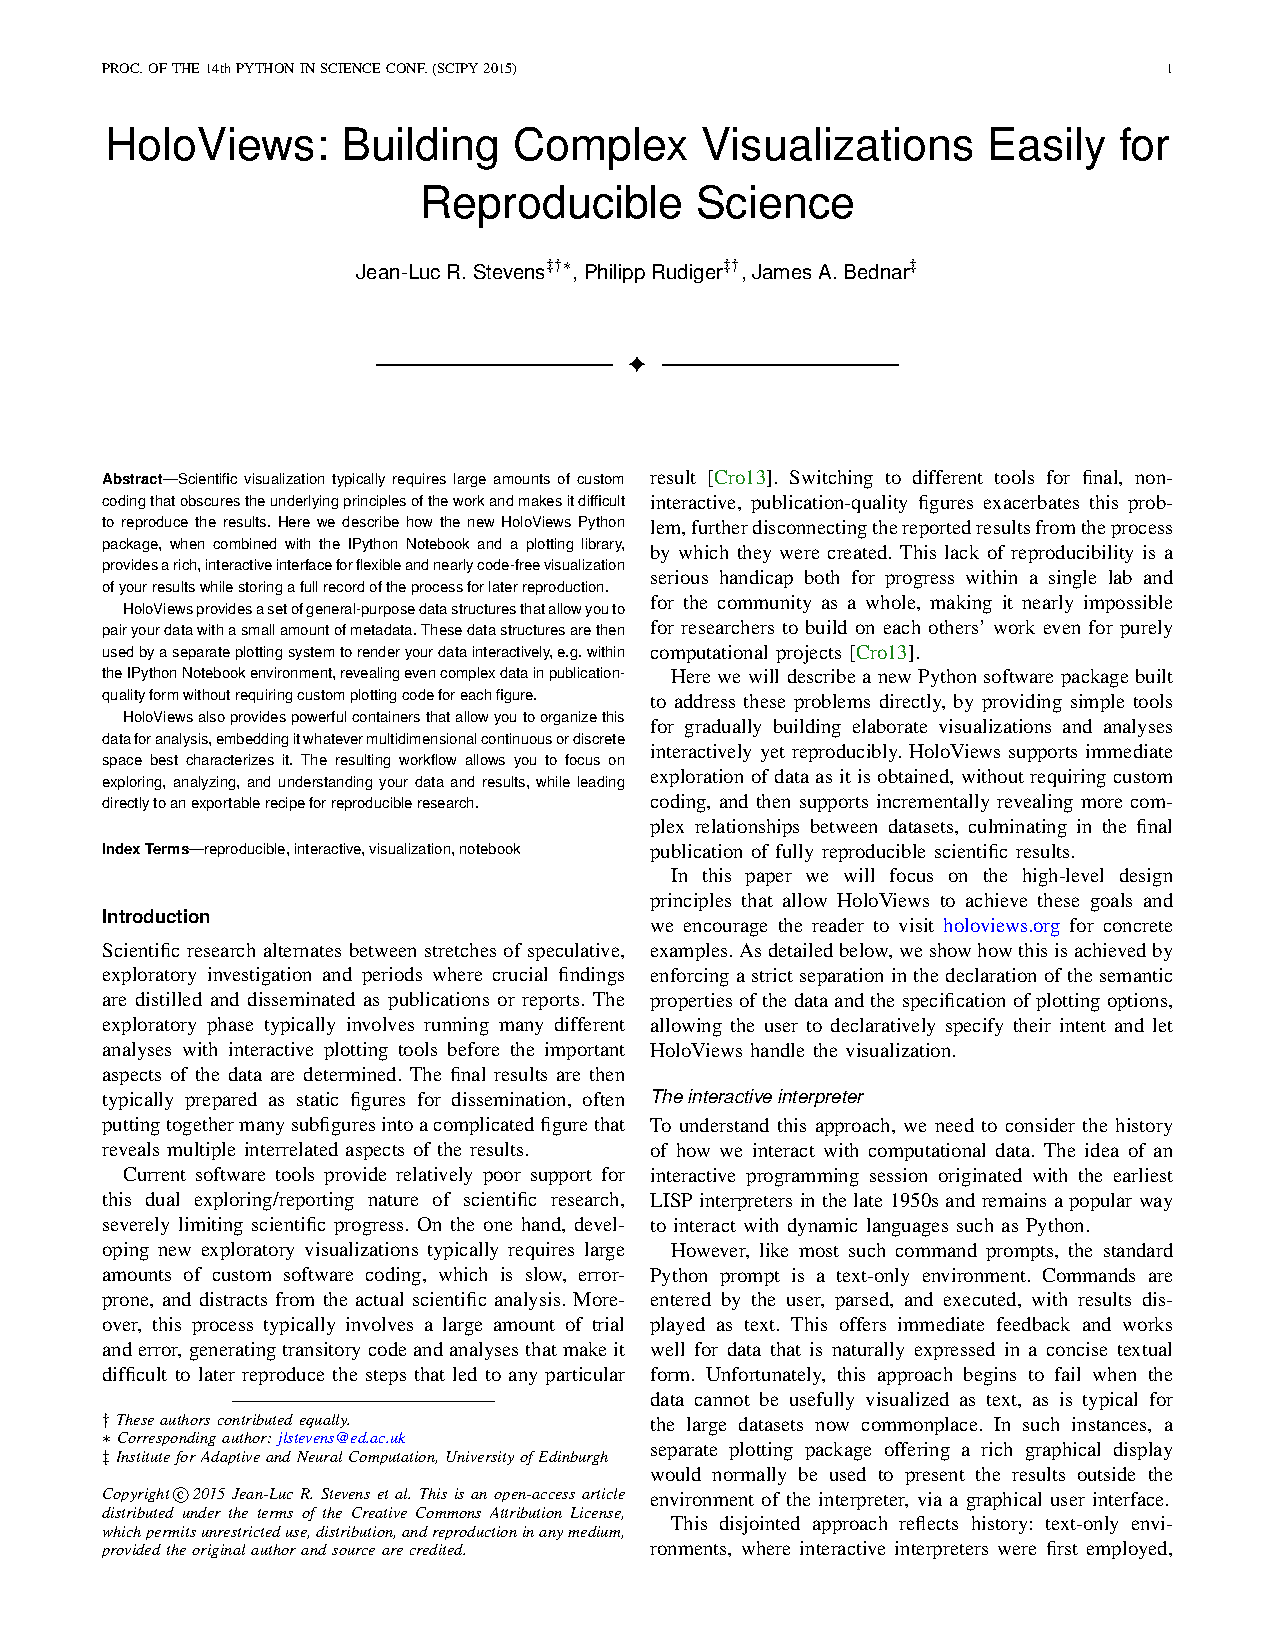
\includepdf[pagecommand={\thispagestyle{headings}}, pages={1-8}, scale=0.95]{HoloViews_SciPy.pdf}

\section{A unified workflow for the analysis of complex computational models}

HoloViews is only a small part of an overall workflow developed as
part of this project in collaboration with a colleague. This section
will describe the overall workflow:

\begin{itemize}
\item IPython notebooks - a reproducible record of your work
\item HoloViews - access to data independent of plotting details
\item Easy data exploration of even large parameter spaces
\item Publication quality figures
\item Cite papers published using HoloViews
\item Reiterate how central all this is to working with complex models
\end{itemize}

\begin{figure}
	\centering
        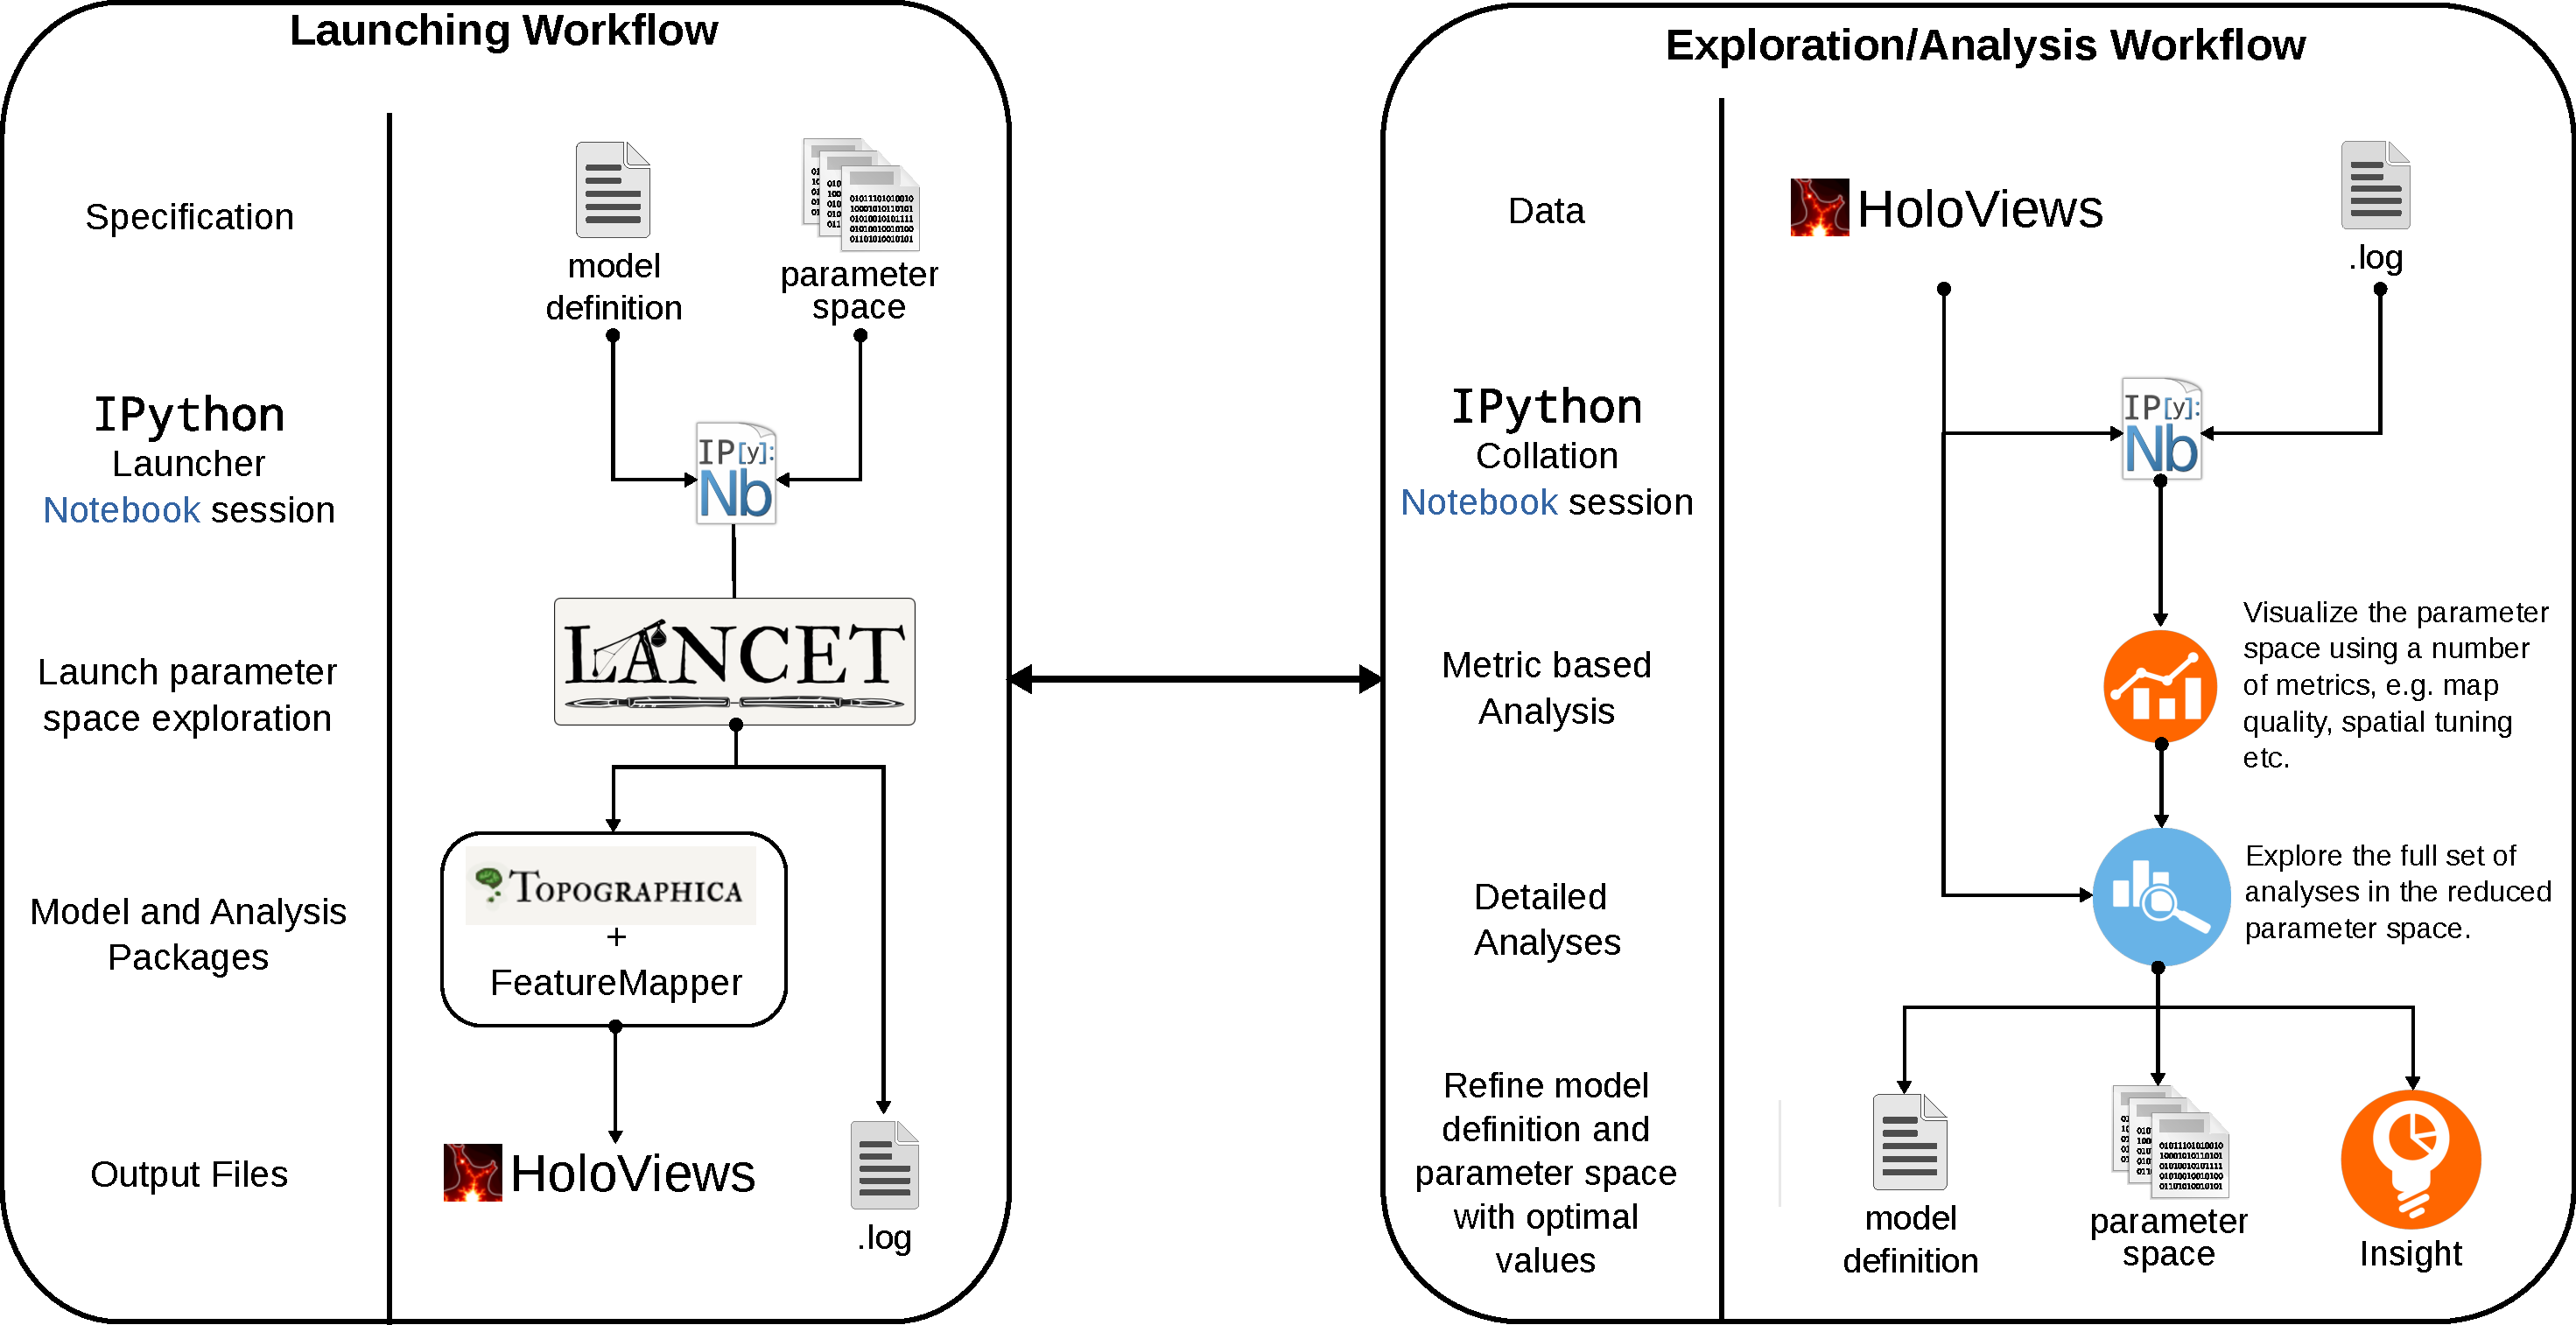
\includegraphics[width=1.0\textwidth]{workflow.pdf}
	\caption{}
	\label{workflow}
\end{figure}




